\documentclass{article}
\usepackage[margin=1.5cm,bottom=2cm]{geometry}
\usepackage{fancyhdr}
\usepackage{graphicx}
\pagestyle{fancy}
\usepackage{enumitem,amssymb,amsmath}
\newlist{todolist}{itemize}{2}
\setlist[todolist]{label=$\square$}
\usepackage{circuitikz}

\begin{document}
	%\fancyhead[L]{ 
\includegraphics[width=2cm]{au_logo.png} }
	\fancyhead[R]{PHYS 2250: General Physics II}
	\fancyfoot[C]{\thepage}
	\vspace*{0cm}
	\begin{center}
		{\LARGE \textbf{Quiz 8}}
		%\vspace{0.25cm}
		%{\Large Due: Friday, September 11}
	\end{center}
	
The following information may or may not be of use:\\
\hrulefill\\
\begin{align*}
	\text{Lorentz Force Law: } \vec{F}&=q\left(\vec{E}+\vec{v}\times\vec{B}\right)\\
	\text{Electrical Power: } P &= I\Delta V\\
\end{align*}

\hrulefill \\
\\

In a region of space there is a uniform magnetic field with magnitude $\left|\vec{B}\right|=5\ \mathrm{T}$ pointing out of the page. A neutral metal bar of length $L=0.2$ m slides horizontally with speed $\left|\vec{v}\right|=500\ \frac{\mathrm{m}}{\mathrm{s}}$ across two fixed conducting rails with negligible friction but good electrical contact. The two metal rails are connected by a resistor with resistance $R=220\ \Omega$.
\begin{center}
	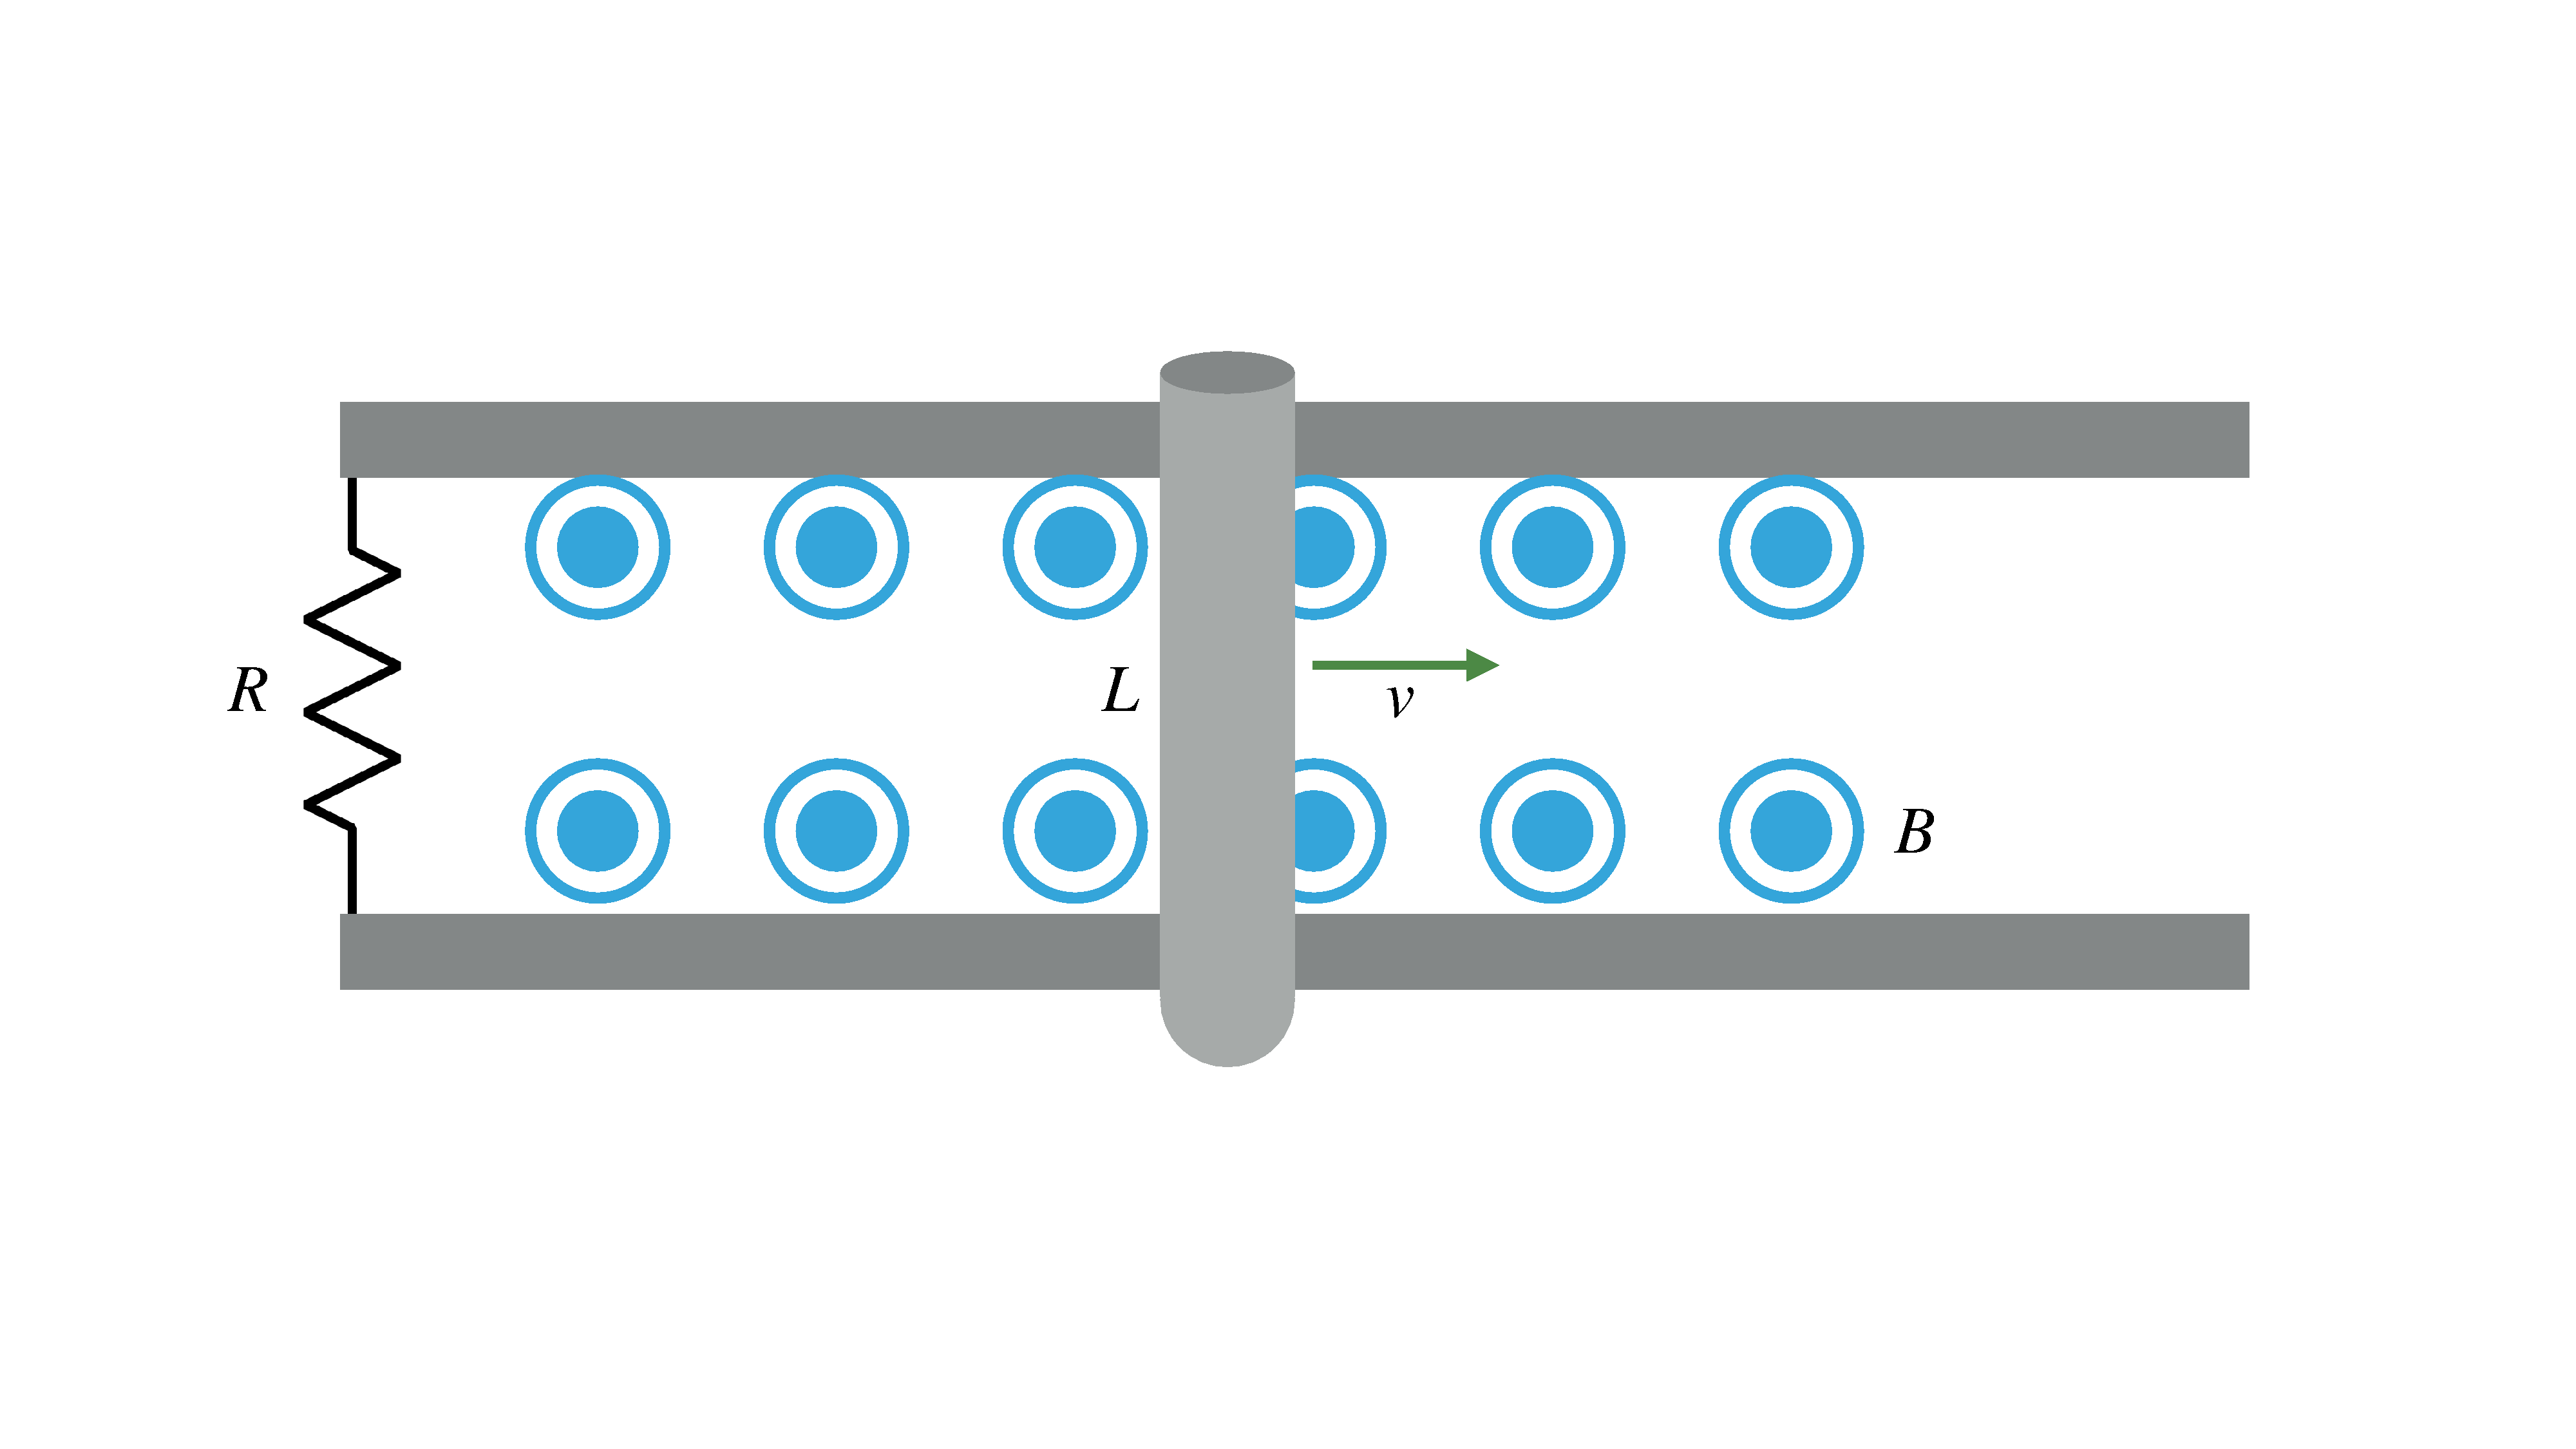
\includegraphics[width=.5\textwidth]{motional_emf}
\end{center}

\begin{enumerate}
	\item What direction is current flowing through the resistor? Indicate by drawing an arrow on the diagram.
	\vspace{1cm}
	\item At this instant, what is the power dissipated in the resistor?
	\vspace{5cm}
	\item The speed of the metal bar will \underline{\hspace{1cm}} with time.
	\begin{enumerate}
		\item Increase
		\item Remain constant
		\item Decrease
	\end{enumerate}
\end{enumerate}
\end{document}